\begin{frame}[t,allowframebreaks,allowdisplaybreaks]
    \subsubsection{Search value}
    \frametitle{B-Tree Operations---Search}
    \vspace{-1cm}
    \begin{columns}
        \begin{column}{\textlecolumn}
            \begin{block}{}
                \begin{itemize}
                    \item The changes of this operations are mainly focused on the search part, since we have to compare to an array of keys and not only the node key.
                    \item This operation returns the object in the B-Tree if a given key exists.
                \end{itemize}
            \end{block}
        \end{column}
        \begin{column}{\textricolumn}
        \end{column}
    \end{columns}
    \inputminted[
        highlightlines={6,12,19,22,27}
    ]{c}{resources/code/b_tree_find.c}
    \begin{figure}[h!]
        \includegraphics[%
            width=0.55\linewidth,%
            page=62%
        ]{resources/made/B-Trees_insert_example.pdf}
    \end{figure}
    \begin{itemize}
        \item Let's search for \(70\) in this \(t\left(2,2\right)\) B-Tree.
    \end{itemize}
\end{frame}
